\chapter{Cazuri de Utilizare}

Definirea cazurilor de utilizare oferă o perspectivă clară asupra funcționalităților oferite de extensie și a interacțiunilor dintre utilizator și sistem. Extensia a fost proiectată pentru 
a automatizarea și îmbunătățirea procesului educațional, prin structurarea conținutului în module parcurse progresiv. Punctul de plecare al studentului este ales prin intermediul unui 
test inițial ce verifică cunoștințele acestuia asupra subiectului. Deciziile privind trecerea de la un modul la altul sunt luate tot în funcție de perfomanța studentului, determinată cu 
ajutorul testelor generate automat din conținutul fișierului încărcat de profesor. Acest comportament oferă o experiență de învățare personalizată și eficientă.

Cazurile de utilizare acoperă două categorii de utilizatori:
\begin{itemize}
    \item \textbf{Profesor}: are rolul de a crea activitatea, de a încărca materialul pe baza căruia este generat conținutul educațional, de a revizui modulele generate și de a urmări progresul studenților.
    \item \textbf{Student}: are rolul de accesa activitatea, de a completa un test ințial, de a urma modulele în ordine și de a rezolva noi teste destinate progresării către următorul modul.
\end{itemize}

\section{Use Case Diagram}
\begin{figure}[H]
    \centering
    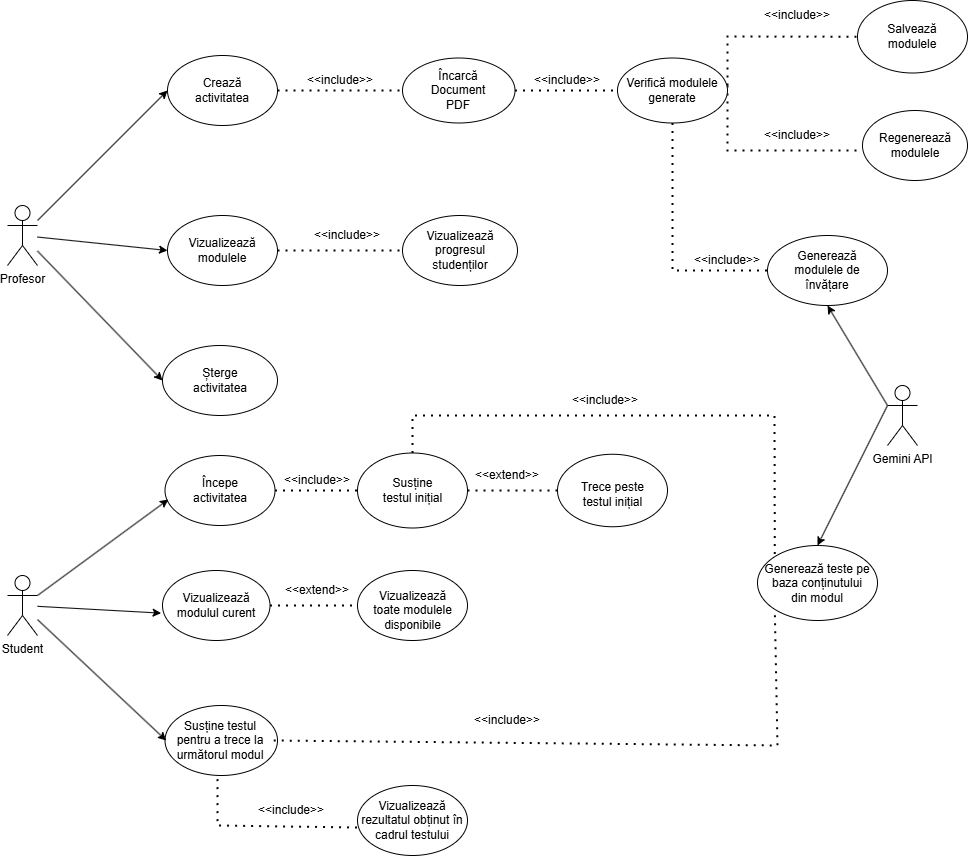
\includegraphics[width=1\textwidth]{images/LicentaUseCase.png}
    \caption{Use Case Diagram}
    \label{fig:use_case_diagram}
\end{figure}

\section{Cazuri de utilizare pentru profesor}

\subsection{Crearea activității}
Profesorul are posibilitatea de a adăuga o activitate nouă de tip \textit{Adaptive Learning} în cadrul unui curs. Activitatea poate fi adăugată în orice secțiune a cursului și se găsește
în lista de activități disponibile. Pentru a crea o activitate, profesorul trebuie să completeze un formular în care specifică numele activității, descrierea acesteia și să încarce un fișier
care conține materialul educațional. Acest fișier va fi folosit ulterior pentru generarea automată a modulelor de învățare. 
\begin{figure}[H]
    \centering
    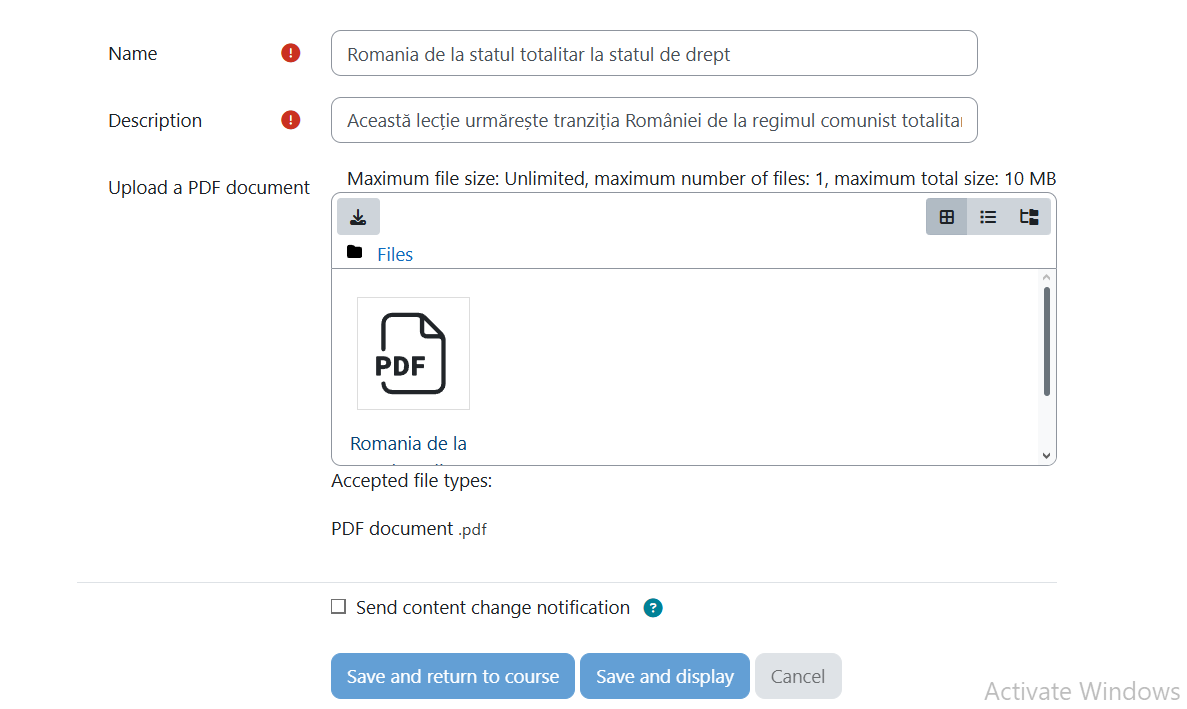
\includegraphics[width=0.8\textwidth]{images/formPage.png}
    \caption{Crearea activității de tip Adaptive Learning}
    \label{fig:creare_activitate}
\end{figure}

\subsection{Revizuirea modulelor generate}
După ce profesorul a încărcat fișierul, extensia va procesa conținutul, generând module de învățare cu ajutorul Gemini API. Profesorul are posibilitatea de a previzualiza modulele generate 
și are opțiunea de a le regenera, dacă consideră că acestea nu sunt conforme cu așteptările sau dacă dorește să facă modificări, și opțiunea de a le salva și publica studenților în cazul în 
care este mulțumit de acestea prin intermediul a două butoane, \textit{Save modules} și \textit{Regenerate modules}.
\begin{figure}[H]
    \centering
    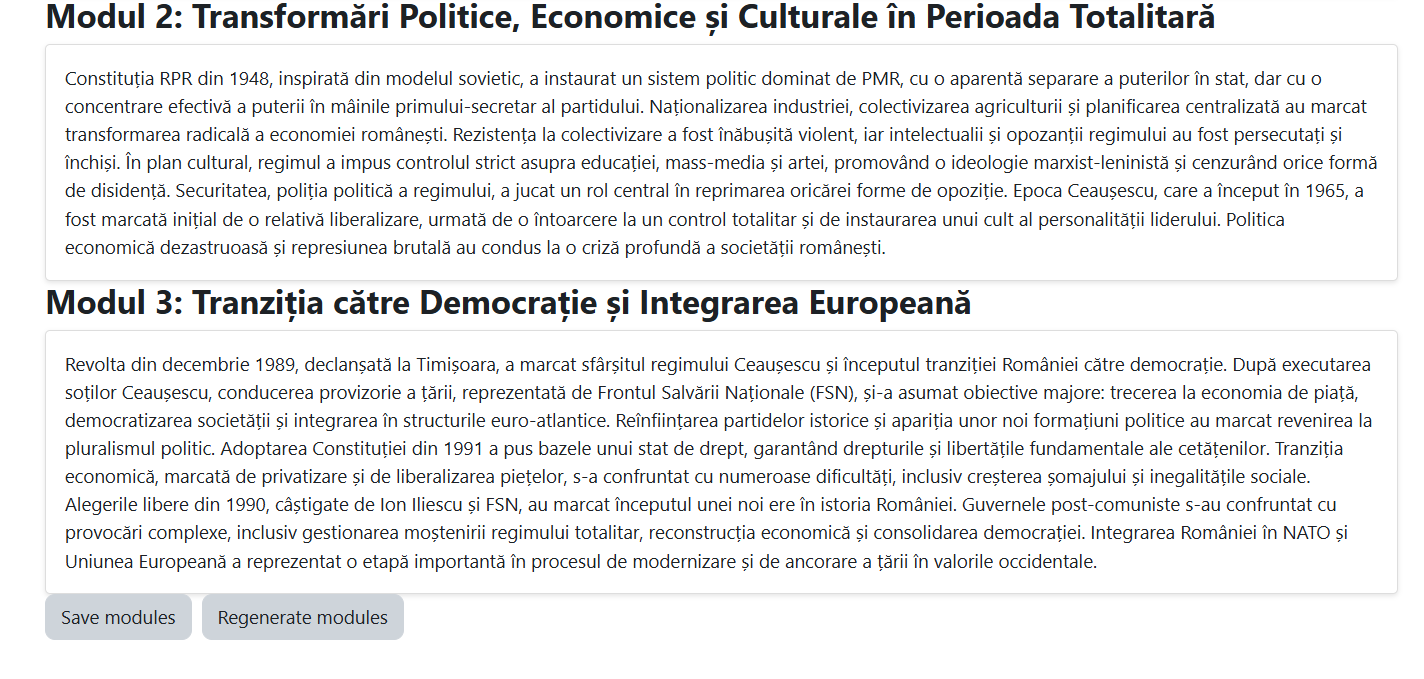
\includegraphics[width=0.8\textwidth]{images/reviewPage.png}
    \caption{Revizuirea modulelor generate}
    \label{fig:revizuire_module}
\end{figure}

\subsection{Vizualizarea modulelor și urmărirea progresului studenților}
După salvarea modulelor, profesorul este redirecționat către pagina de vizualizare a modulelor, pagină ce poate fi accesată și ulterior din meniul cursului. Pe această pagină, profesorul 
poare vedea lista modulelor generate, cu titlul și conținutul lor. De asemenea, acesta area acces la un tabel unde poate vedea progresul studenților. Tabelul conține numele complet al 
studentului, în format \textit{Prenume Nume}, Titlul și numărul modulului la care se află și ziua, data și ora la care a început modulul.
\begin{figure}[H]
    \centering
    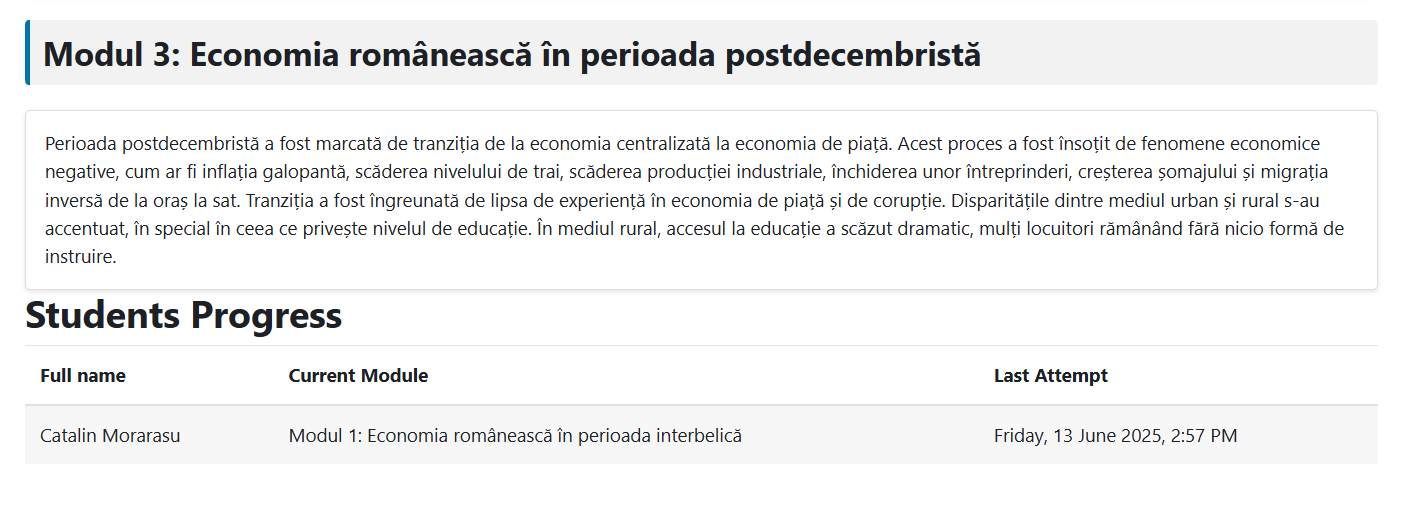
\includegraphics[width=0.9\textwidth]{images/viewProgressPage.png}
    \caption{Vizualizarea modulelor și urmărirea progresului studenților}
    \label{fig:vizualizare_module}
\end{figure}

\subsection{Ștergerea activității}
Profesorul are posibilitatea de a șterge activitatea de tip \textit{Adaptive Learning} din curs. Această acțiune va elimina toate modulele generate și progresul studenților asociat cu
această activitate. Ștergerea activității se realizează similiar cu ștergerea oricărei alte activități din Moodle, prin intermediul butonului \textit{Delete} disponibil în meniul de 
administrare al cursului, meniu accesibil doar utilizatorilor cu rol de profesor sau administrator ce se află în modul editare.

\section{Cazuri de utilizare pentru student}
\subsection{Începerea activității}
Pentru student, activitățile de tip \textit{Adaptive Learning} sunt afișate în lista de activități a cursului. Când studentul accesează activitatea pentru prima dată, acesta este 
redirecționat la pagina de start a activității, unde vede titlul activității, și o descriere a activităților de tip \textit{Adaptive Learning}. Butonul \textit{Start Learning} este 
disponibil pentru a începe activitatea și pentru a trece la testul inițial.
\begin{figure}[H]
    \centering
    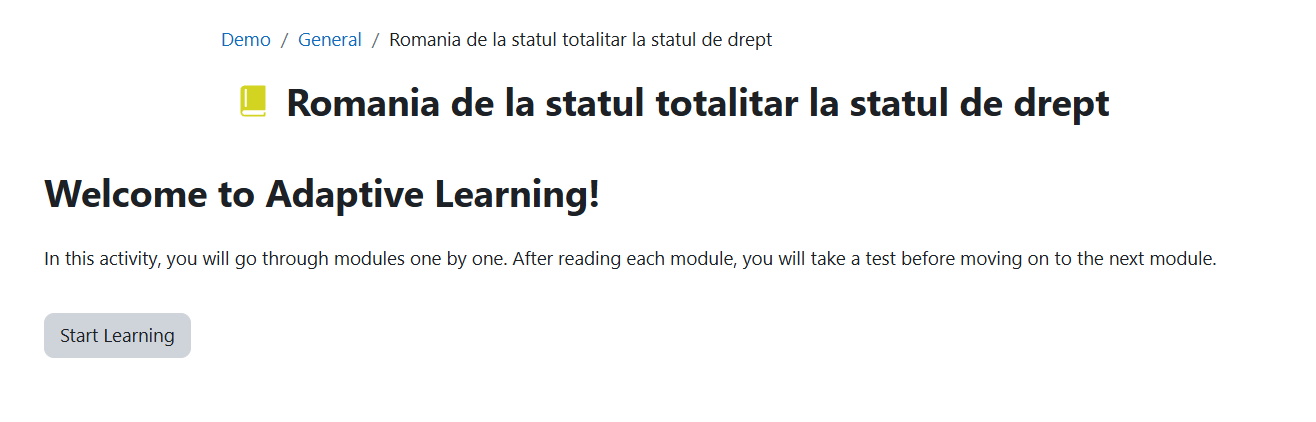
\includegraphics[width=0.8\textwidth]{images/startPage.png}
    \caption{Pagina de start a activității de tip Adaptive Learning}
    \label{fig:pagina_start}
\end{figure}

\subsection{Completarea testului inițial}
După ce studentul apasă butonul \textit{Start Learning}, acesta este redirecționat către pagina de test inițial ce conține întrebări din materialul educațional încărcat de profesor.
Testul inițial este generat automat de Gemini API și are rolul de a evalua cunoștințele studentului asupra subiectului. Prima oară studentul primește un test cu întrebări doar din primul 
modul, iar dacă acesta obține un scor mai mare sau egal cu 75\% va putea accesa testul următorului modul. Dacă studentul nu obține un scor suficient de mare, acesta va rămâne
la același modul și va fi redirecționat către pagina de vizualizare a modulului. În cadrul fiecărui test, studentul are posibiliatea de a trece peste test cu ajuorul butonului 
\textit{Skip test}, caz în care va fi redirecționat către pagina de vizualizare a modulului pentru care era destinat testul. Testul nu are un numărl fix de întrebări, API-ul generând
câte întrebări consideră că sunt necesare pentru a evalua cunoștințele studentului și a cuprinde toate conceptele importante din modulul respectiv, iar fiecare întrebare are patru variante 
de răspuns, dintre care doar una este corectă. După ce studentul a răspuns la toate întrebările, acesta apasă butonul \textit{Submit test} pentru a trimite răspunsurile.
\begin{figure}[H]
    \centering
    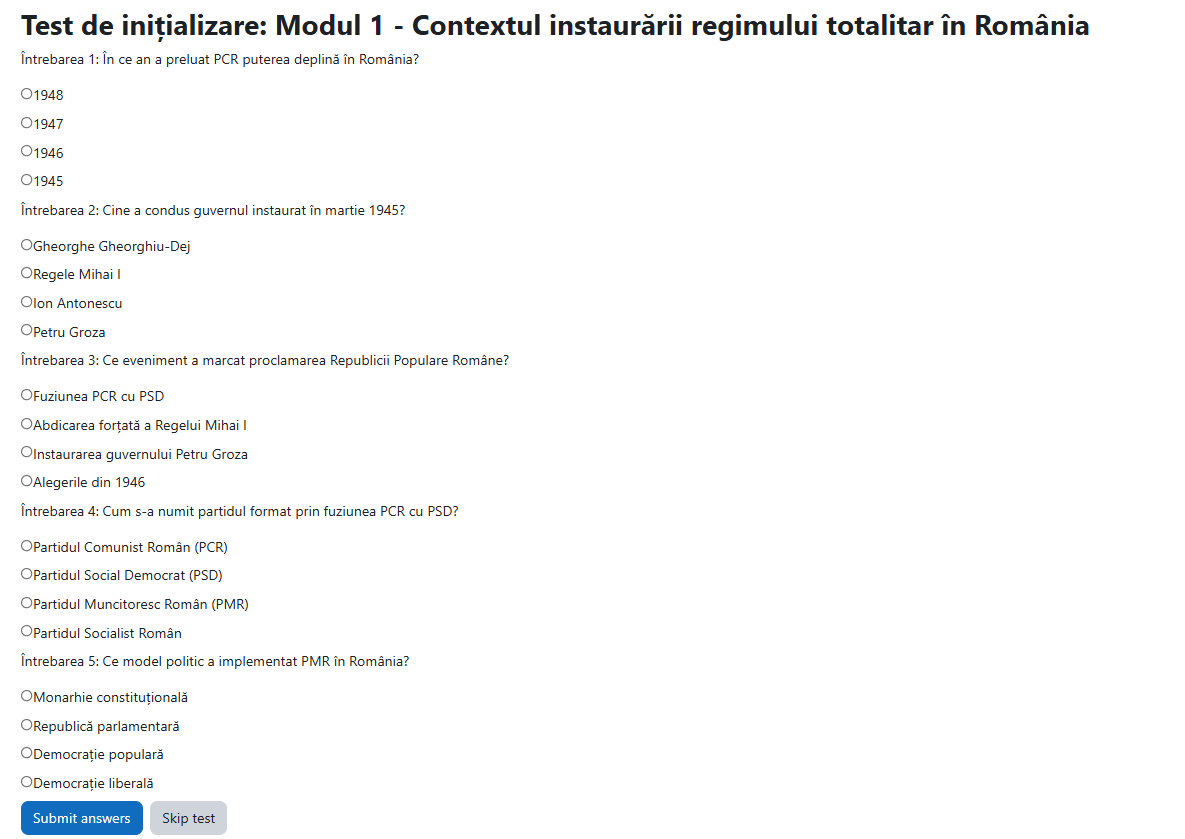
\includegraphics[width=0.9\textwidth]{images/testInit.png}
    \caption{Pagina de test inițial}
    \label{fig:pagina_test_initial}
\end{figure}

\subsection{Vizualizarea modulelor}
După completarea testului inițial, studentul este redirecționat către pagina de vizualizare a modulului curent, pagina fiind accseibilă și ulterior din meniul cursului. Pe această pagină,
studentul poate vedea titlul și conținutul modulului curent. De asemenea, studentul are la îndemână două butoane: \textit{Take Test} și \textit{See available modules}. Butonul 
\textit{Take Test} îl redirecționează către pagina de test pentru modulul curent, iar butonul \textit{See available modules} îl redirecționează către pagina de vizualizare a tuturor
modulelor disponibile, adică cele prin care deja a trecut și cel curent.
\begin{figure}[H]
    \centering
    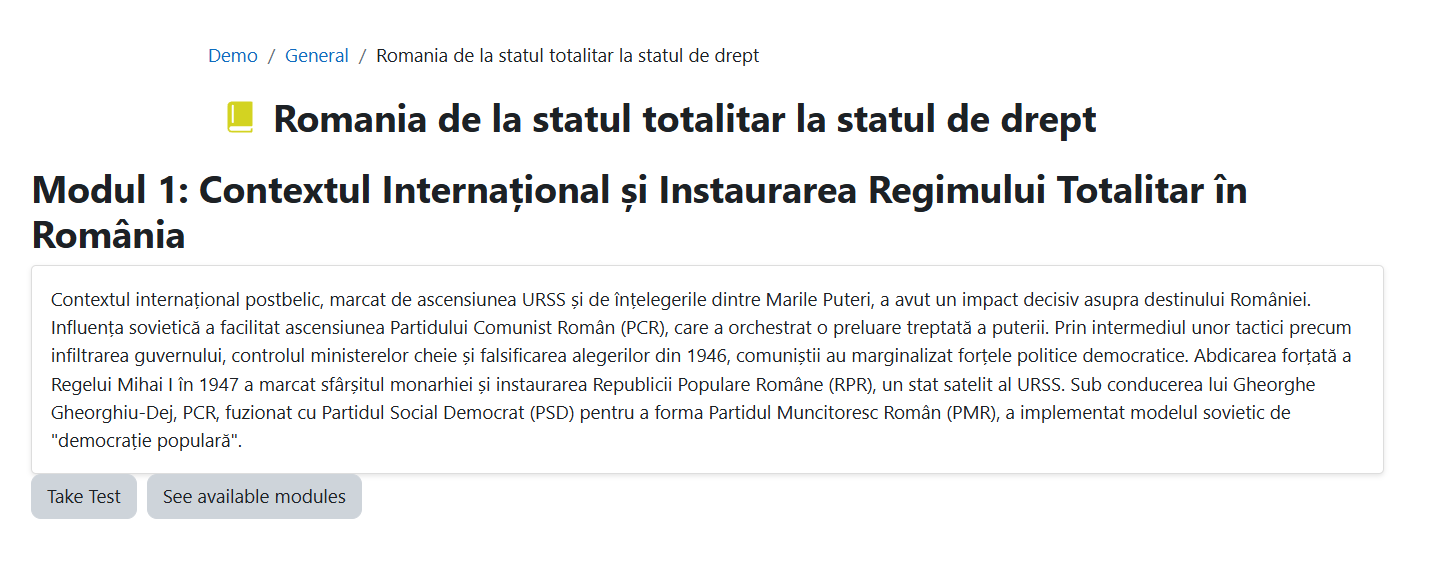
\includegraphics[width=0.8\textwidth]{images/learnPage.png}
    \caption{Pagina de vizualizare a modulului curent}
    \label{fig:vizualizare_modul_curent}
\end{figure}

\subsection{Completarea testului pentru a trece la următorul modul}
După ce studentul a citit conținutul modulului curent, acesta poate accesa testul asociat cu modulul respectiv prin intermediul butonului \textit{Take Test}. Testul este generat automat de 
Gemini API și conține întrebări din materialul educațional al modulului curent. Similar cu testul inițial, acesta nu are un număr fix de întrebări, iar fiecare întrebarea are patru variante 
de răspuns, dintre care doar una este corectă. După ce studentul a răspuns la toate întrebările, acesta apasă butonul \textit{Submit test} pentru a trimite răspunsurile și este redirecționat 
la pagina unde poate vedea rezultatul obținut la test.
\begin{figure}[H]
    \centering
    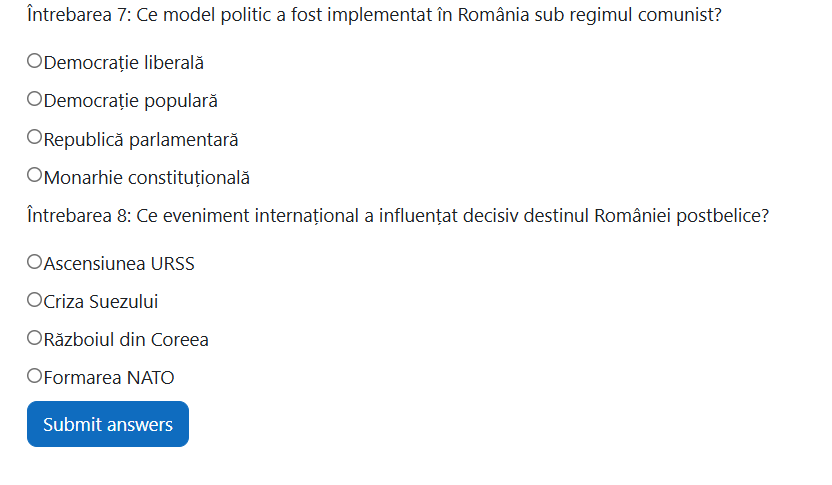
\includegraphics[width=0.7\textwidth]{images/testPage.png}
    \caption{Pagina de test pentru modulul curent}
    \label{fig:pagina_test_modul_curent}
\end{figure}

\subsection{Vizualizarea rezultatului obținut la test}
După ce studentul a trimis răspunsurile la test, acesta este redirecționat către pagina de vizualizare a rezultatului obținut. Aici, studentul vede toate întrebările, răspunsurile sale și 
răspunsurile corecte. De asemenea studentul vede și scorul obținut la test, iar dacă acesta este mai mare sau egal cu 50\% + 1, studentul promovează la următorul modul. Indiferent de 
rezultatul obținut, butonul \textit{Continue learning} trimite studentul la pagina de vizualizare a aceluiași modul dacă nu a promovat, sau la pagina de vizualizare a următorului 
modul dacă a promovat.
\begin{figure}[H]
    \centering
    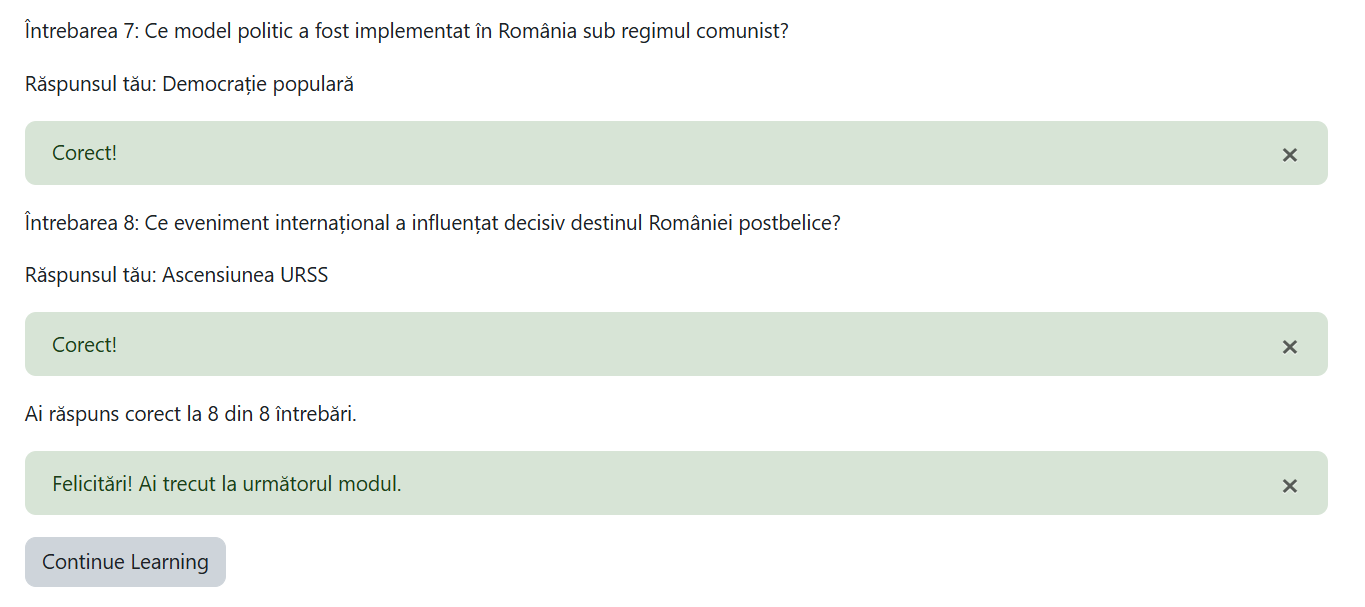
\includegraphics[width=0.8\textwidth]{images/resultPage.png}
    \caption{Pagina de vizualizare a rezultatului obținut la test}
    \label{fig:pagina_rezultat_test}
\end{figure}
\subsection{Vizualizarea tuturor modulelor disponibile}
Pe pagina de vizualizare a modulului curent, studentul are posibilitatea de a accesa pagina de vizualizare a tuturor modulelor disponibile prin intermediul butonului 
\textit{See available modules}. Pagina afișează toate modulele prin care studentul deja a trecut, precum și cel curent. Fiecare modul are titlul și conținutul său, iar pentru a se intoarce 
la modulul curent studentul poate apăsa butonul \textit{Back}.
\begin{figure}[H]
    \centering
    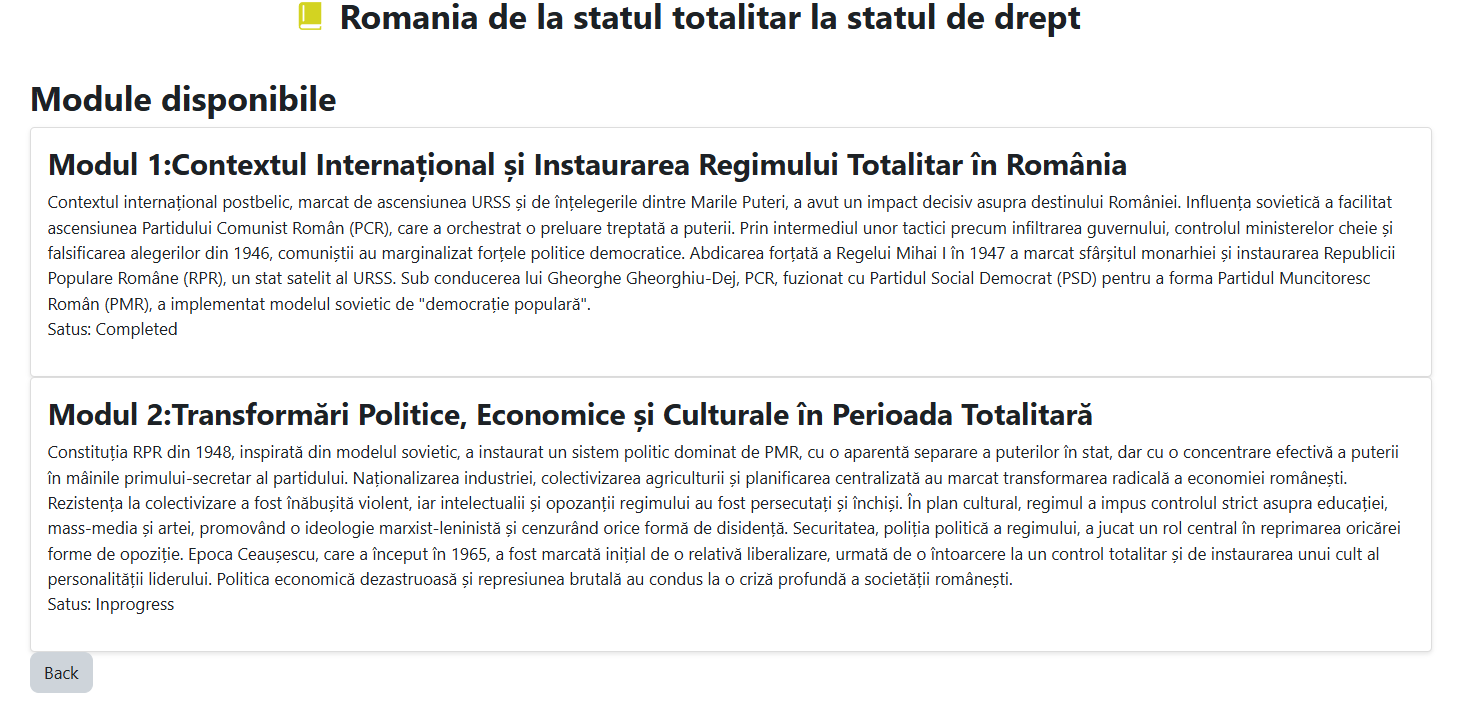
\includegraphics[width=0.8\textwidth]{images/allModulesPage.png}
    \caption{Pagina de vizualizare a tuturor modulelor disponibile}
    \label{fig:pagina_vezi_module}
\end{figure}
\subsection{Finalizarea activității}
După ce studentul a parcurs toate modulele disponibile, acesta este trimis la pagina de finalizare a activității, unde poate vedea un mesaj de felicitare și un buton care îl redirecționează 
la pagina de vizualiarea a tuturor modulelor disponibile, în cazul de față toate modulele din cadrul activității. Studentul poate accesa această pagină și ulterior, din meniul cursului.
\begin{figure}[H]
    \centering
    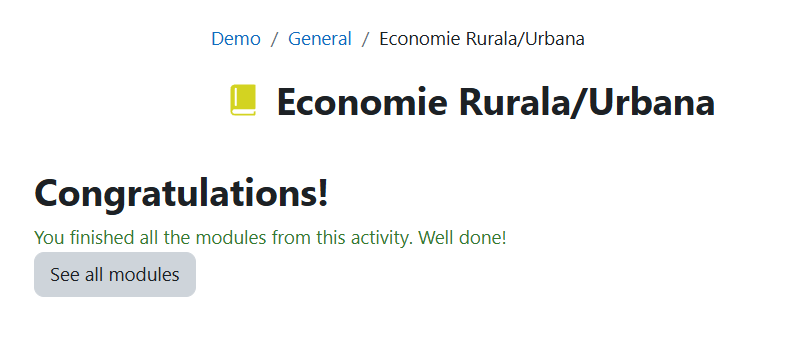
\includegraphics[width=0.8\textwidth]{images/finishPage.png}
    \caption{Pagina de finalizare a activității}
    \label{fig:pagina_finalizare_activitate}
\end{figure}